\section{Navigation}

There are various means of navigating through Murcs. The primary method is to select items from the side bar that you wish to inspect. If you wish to inspect a different item type then the choice box above the side bar may be used to inspect different elements.

\begin{figure}[H]
\centering
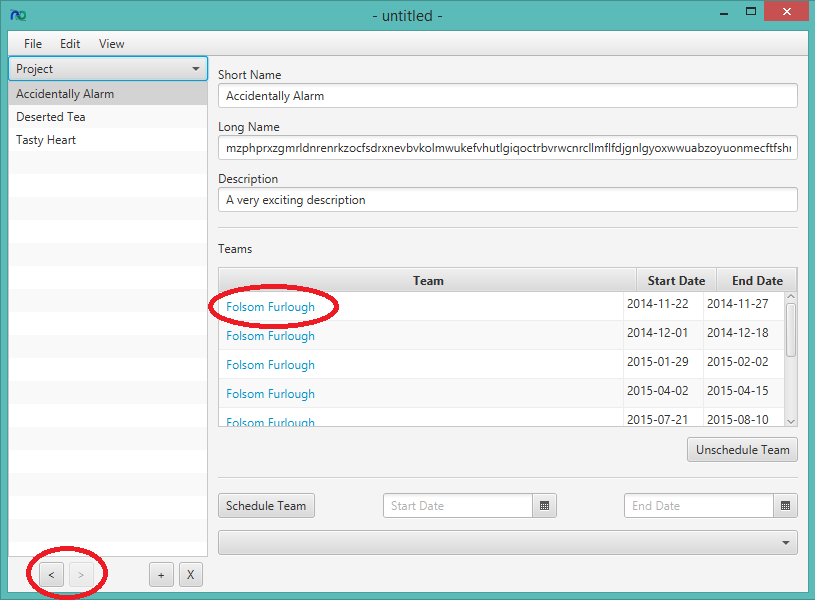
\includegraphics[width=\textwidth]{images/screenshots/navigation.PNG}
\caption{Methods of Navigation}
\label{fig:new_project}
\end{figure}

In order to conveniently go back to previously selected items, there are backward and forward buttons positioned below the side bar that take the application to the previous page. This works up to a maximum of five places. If the undo feature is used then position information will be lost.

In addition to these, when an item is mentioned within another items editor, it exists as a hyperlink to that items editor window.

It is also possible to go back and forward by holding the ALT key and pressing the LEFT and RIGHT arrow.